
\documentclass{beamer}

\usepackage{algpseudocode, color, colortbl, listings, MnSymbol}

\usepackage{hyperref}
\hypersetup{
    colorlinks=true,
    urlcolor=blue,
}

\usetheme{Montpellier}
\usecolortheme{rose}

% page numbers, from
% https://tex.stackexchange.com/questions/137022/how-to-insert-page-number-in-beamer-navigation-symbols
\expandafter\def\expandafter\insertshorttitle\expandafter{%
  \insertshorttitle\hfill%
  \insertframenumber\,/\,\inserttotalframenumber}

\definecolor{Gray}{gray}{0.8}
\newcolumntype{g}{>{\columncolor{Gray}}c}

\newcommand{\stanza}{ \\~\ }

\title{15. Approximate Set Cover and Bin Packing}
\subtitle{CPSC 535}
\author{Kevin A. Wortman}
\institute{ 
\includegraphics[height=2cm]{csuf-logo-cmyk} }
\date{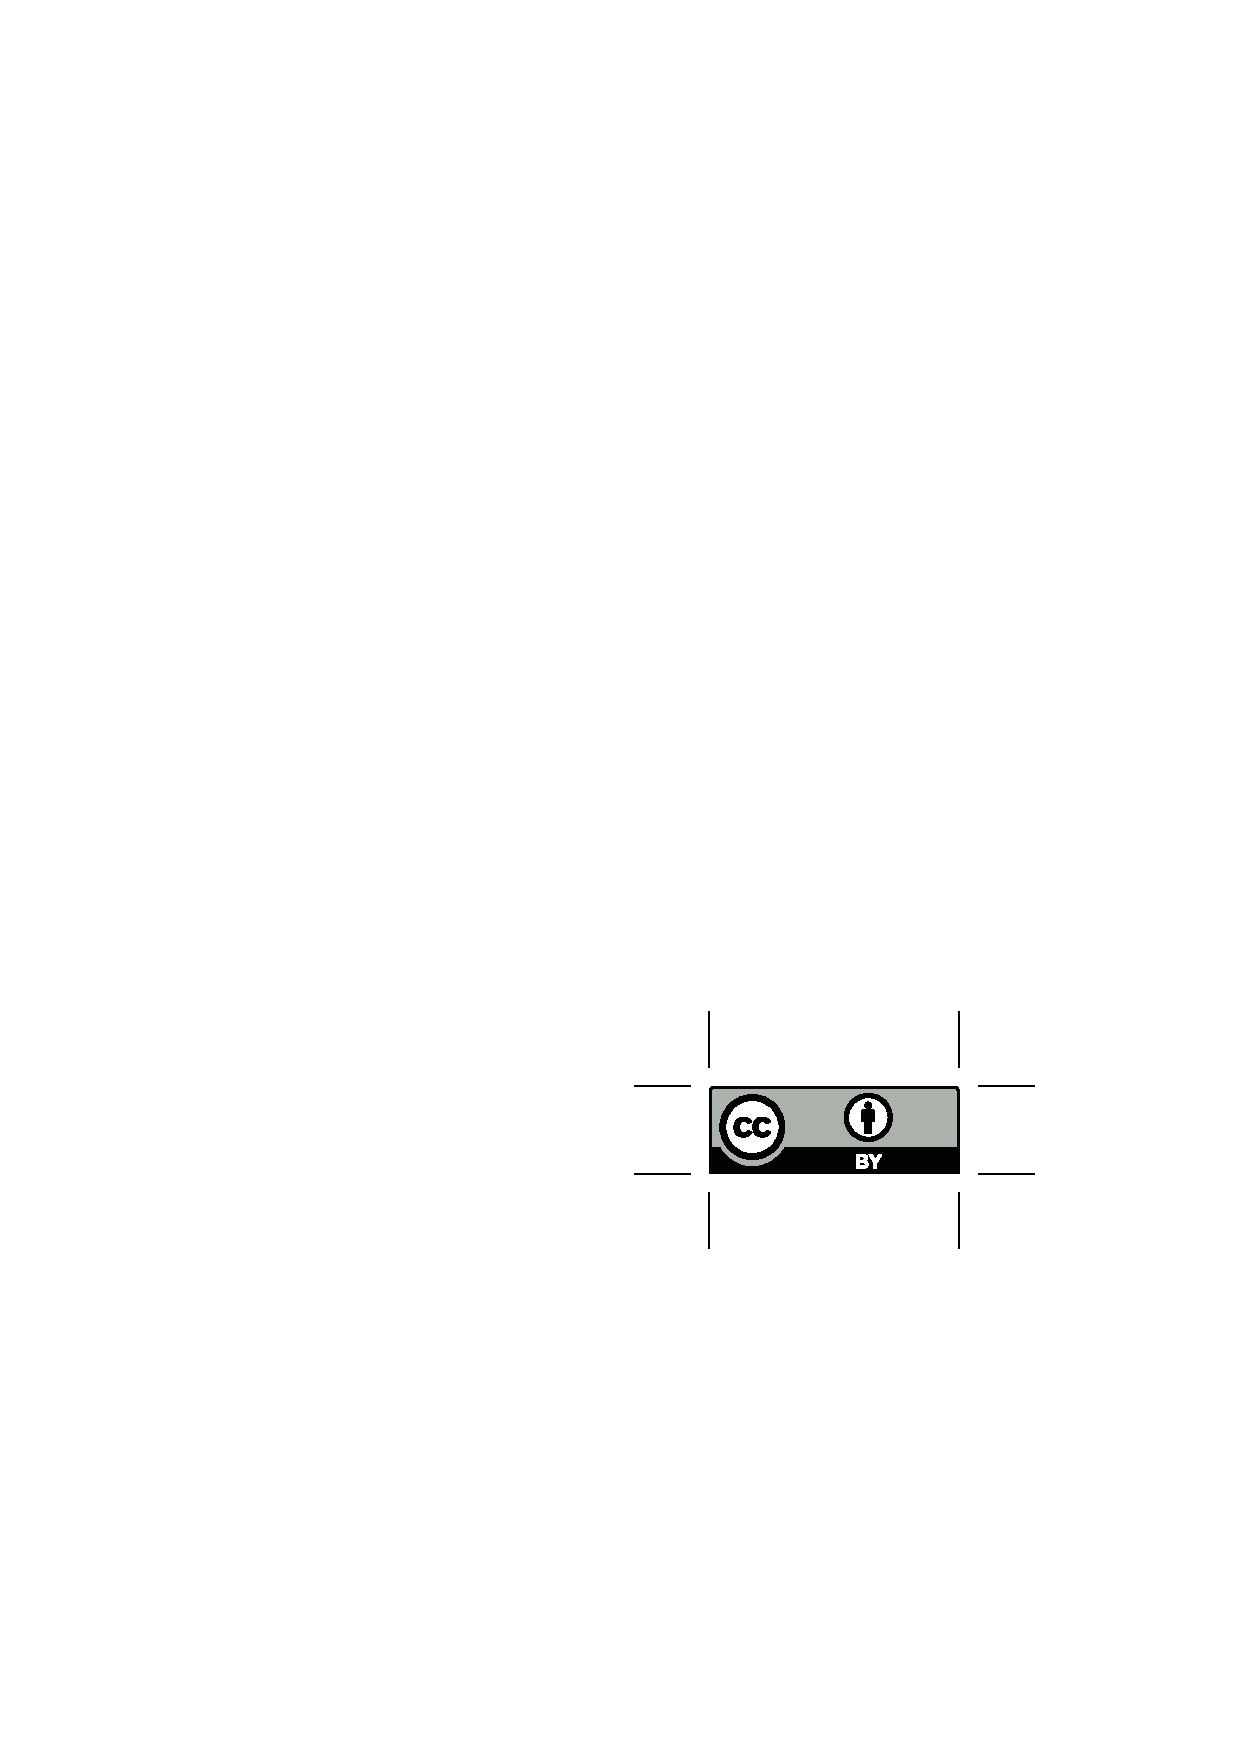
\includegraphics[height=14pt]{by} \\

{\tiny
This work is licensed under a
\href{http://creativecommons.org/licenses/by/4.0/}{Creative Commons Attribution 4.0 International License}.
}}

\begin{document}

\begin{frame}
  \titlepage
\end{frame}

\begin{frame} \frametitle{Set Cover: Intuition}
\begin{itemize}
  \item list of \textbf{needs}
  \item list of \textbf{services}
  \begin{itemize}
    \item each service meets some of the needs
  \end{itemize}
  \item \textbf{puzzle:} shortest list of products that meets all the needs?
\end{itemize}
\end{frame}

\begin{frame} \frametitle{Set Cover: Formal Definition}
  \emph{set cover problem} \\
  \textbf{input}: a universe set $X,$ and family $\mathfrak{F}$ of subsets of $X,$ such that $X=\bigcup_{S \in \mathfrak{F}} S$ \\
  \textbf{output}: a minimum size subfamily $\mathfrak{C} \subseteq \mathfrak{F}$ whose members cover all of $X,$ so
    $X = \bigcup_{S \in \mathfrak{C}} S$
\end{frame}

\begin{frame} \frametitle{Application: Streaming Services}
\begin{itemize}
  \item \textbf{needs:} stream TV shows $A, B, C, D, E, F$
  \item $X = \{A, B, C, D, E, F\}$
  \item \textbf{services:} alternative streaming services; each offer only some shows
  \item $\mathfrak{F} = \{ \{ A, F \}, \{A, C, E\}, \{B, E \}, \ldots \}$ 
  \item \textbf{puzzle:} subscribe to smallest number of services that provide all desired shows
\end{itemize}
\end{frame}

\begin{frame} \frametitle{Application: Menu Design}
  \begin{itemize}
    \item \textbf{needs:} menu has a food option available for various dietary needs
    \item $X = \{carnivore, vegan, kosher, halal, glutenfree, \ldots \}$
    \item \textbf{services:} alternative entrees
    \item $\mathfrak{F} = \{ \{ carnivore, halal \}, \{vegan\}, \{kosher, carnivore\}, \ldots \}$ 
    \item \textbf{puzzle:} design a menu with the fewest number of food options so that everyone can eat something
  \end{itemize}
\end{frame}
  
\begin{frame} \frametitle{Set Cover Hardness}
  \begin{itemize}
    \item set cover is $NP$-complete
    \item baseline algorithm: for each subset $\mathfrak{C} \subseteq \mathfrak{F},$ check if the sets in $\mathfrak{C}$ contain all elements, keep track of the smallest such $\mathfrak{C}$
    \item $\Theta(2^n \cdot n)$ time, slow
  \end{itemize}
\end{frame}

\begin{frame} \frametitle{Set Cover Approximation Algorithm}
  \begin{algorithmic}[1]
    \Function{APPROX-SET-COVER}{$X, \mathfrak{F}$}
      \State $U_0=\emptyset$ \Comment{still-uncovered elements}
      \State $\mathfrak{C} = \emptyset$
      \State $i=0$
      \While { $U_i \ne \emptyset$ }
        \State // choose set with most currently-uncovered elements
        \State Find $S \in \mathfrak{F}$ that maximizes $|S \cap U_i|$  
        \State $U_{i+1} = U_i - S$
        \State $\mathfrak{C} = \mathfrak{C} \cup \{S\}$
        \State $i = i + 1$
      \EndWhile
      \State \Return $\mathfrak{C}$
    \EndFunction
  \end{algorithmic}
\end{frame}

\begin{frame} \frametitle{Efficiency Analysis}
  \begin{itemize}
    \item while loop: $\Theta(n)$ iterations
    \begin{itemize}
      \item Find: $\Theta(n)$ time (assuming fast data structure to look up $U_i$)
      \item $U_{i+1} = U_i - S$: $\Theta(n)$ time
    \end{itemize}
    \item other steps: $\Theta(1)$ time each
    \item total time $\Theta(n^2)$ 
    \item can be sped up to $\Theta(n)$ (CLRS Exercise 35.3-3)
  \end{itemize}
\end{frame}

\begin{frame} \frametitle{Approximation Ratio}
\textbf{Theorem:} APPROX-SET-COVER is a $O(\lg n)$-approximation algorithm

Proof sketch:
\begin{itemize}
  \item Let $\mathfrak{C}^\star$ be the optimal cover and $k=|\mathfrak{C}$
  \item $\mathfrak{C}$ covers all of $X,$ and each $U_i \subseteq X$, so $\mathfrak{C}^\star$ covers every $U_i$
  \item each $U_i$ can be covered with $\leq k$ sets from $\mathfrak{F}$
  \item on average, $\mathfrak{C}^\star$ covers $n/k$ elements/set
  \item so at least one set in $\mathfrak{F}$ covers $\geq n/k$ elements
  \item APPROX-SET-COVER picks the set that covers the most elements, so each $S$ covers at least $n/k$ additional elements,
    and \[ U_{i+1} \leq |U_i| - |U_i|/k = |U_i|(1-1/k) \]
\end{itemize}
\end{frame}

\begin{frame} \frametitle{Approximation Ratio (continued)}
  \[ U_{i+1} \leq |U_i|(1-1/k) \]
  \begin{itemize}
    \item algorithm stops when some $|U_i|=0$
    \item as a recurrence,
      \[ T(n) = (1-1/k)n \]
    \item algebra and log rules show $T(n) \in O(k \lg n)$
    \item each iteration adds one set to $\mathfrak{C}$, so APPROX-SET-COVER picks $O(k \lg n)$ sets
    \item $k$ is the optimal number of sets, so
    \item $\therefore$ APPROX-SET-COVER is a $O(\lg n)$-approximation algorithm $\qedsymbol$
  \end{itemize}
  \end{frame}
  
\begin{frame} \frametitle{Set Cover Summary}
\begin{itemize}
  \item set cover is $NP$-complete, exact algorithm takes exponential time
  \item fast $O(\lg n)$-approximate algorithm
  \item showed $\Theta(n^2)$ time
  \item $\Theta(n)$ time is possible
\end{itemize}
\end{frame}

\begin{frame} \frametitle{Big Idea: Linear Programming Relaxation}
Recall:
\begin{itemize}
  \item linear programming with real-valued variables is fast (polynomial time)
  \item integer linear programming (MIP) is $NP$-complete and slow (exponential time)
\end{itemize}

Idea:
\begin{itemize}
  \item formulate our problem as a MIP
  \item ``cheat'' and solve it as a LP
  \item round off each solution variable to the nearest integer
\end{itemize}
\end{frame}

\begin{frame} \frametitle{Big Idea: Linear Programming Relaxation}
\begin{itemize}
  \item \textbf{LP relaxation:} MIP formulation where no variables are required to be integer
  \item not correct in general
  \item \textbf{but,} sometimes we can prove an approximate performance ratio
  \item next: algorithm that uses LP relaxation to solve vertex cover
\end{itemize}
\end{frame}

\begin{frame} \frametitle{Review: Vertex Cover}
  \emph{vertex cover problem} \\
  \textbf{input}: undirected graph $G=(V,E)$ \\
  \textbf{output}: set of vertices $C \subseteq V$, of minimal size $|C|,$ such
    that every edge in $E$ is incident on at least one vertex in $C$
   \stanza
  \begin{itemize}
    \item $NP$-complete
    \item previous slides: greedy algorithm, 2-approximate, $\Theta(m+n)$ time
    \item goal: better performance ratio (smaller)
    \item expect algo. to be more complicated, slower, or both
  \end{itemize}
\end{frame}

\begin{frame} \frametitle{Vertex Cover Example}
  \begin{center}
    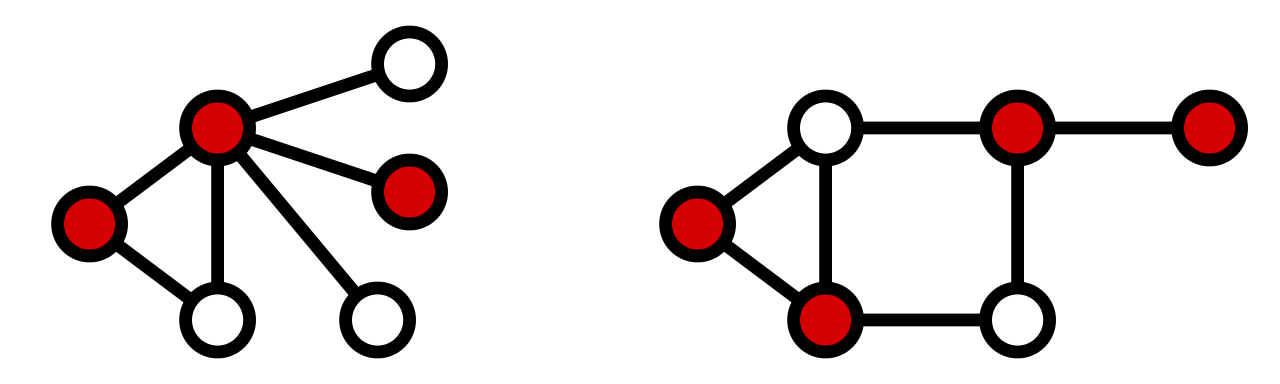
\includegraphics[height=80pt]{13-vertex-cover-1.png}
    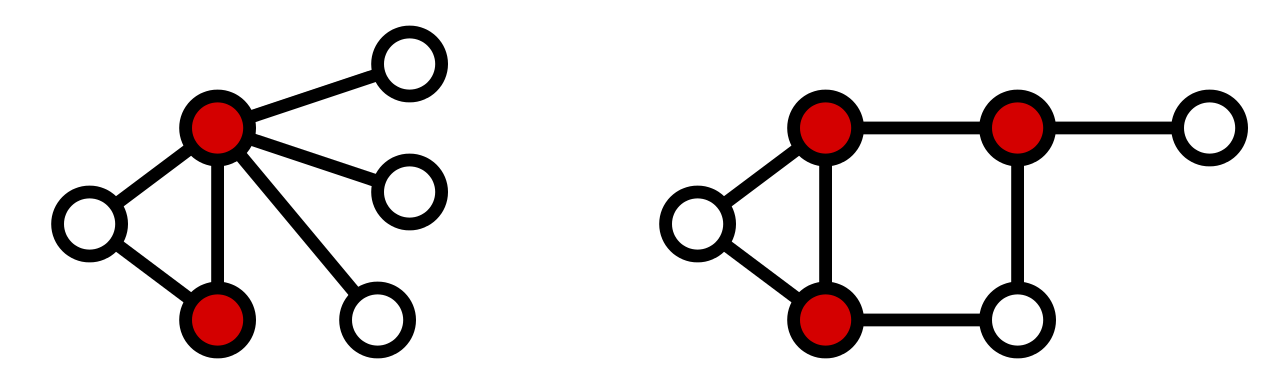
\includegraphics[height=80pt]{13-vertex-cover-2.png}
  \end{center}

  {\tiny
  Images credit: Wikipedia user Miym,
  \href{https://creativecommons.org/licenses/by-sa/3.0)}{CC BY-SA 3.0},
  \url{https://commons.wikimedia.org/wiki/File:Vertex-cover.svg},
  \url{https://commons.wikimedia.org/wiki/File:Minimum-vertex-cover.svg}
  }
\end{frame}

\begin{frame} \frametitle{Review: Formulating Vertex Cover}
  \textbf{Variables:} for each $v \in V$, create an integer variable $x_v$ such that
  \[ x_v = 1 \Leftrightarrow v \in C \]
  
  \textbf{Objective:} minimize
  \[ \sum_{v \in V} x_v \]
  
  \textbf{Constraints:}
  \begin{tabular}{lll}
    $0 \leq x_v \leq 1$ & $\forall v \in V$ & (0 or 1 indicator) \\
    $x_u + x_v \geq 1$ & $\forall (u, v) \in E$ & (each edge is covered)
  \end{tabular}
  
\end{frame}

\begin{frame} \frametitle{Review: Vertex Cover Outcomes}
  \begin{itemize}
    \item \textbf{Infeasible:}
      \begin{itemize}
      \item never happens
      \item $\exists$ a solution: setting all $x_v=1$ satisfies all constraints
      \end{itemize}
    \item \textbf{Unbounded:}
    \begin{itemize}
      \item never happens
      \item objective is bounded: the objective function is to minimize 
        \[ \sum_{v \in V} x_v; \]
        since every $x_v \geq 0$, the minimum objective value is zero, which is finite, so the program is never unbounded
    \end{itemize}
    \item \textbf{Solution:} Construct $C$ as
      \[ C = \{ v \,|\, v \in V \text{ and } x_v=1 \} \]
    \end{itemize}
\end{frame}

\begin{frame} \frametitle{Vertex Cover LP Relaxation}
  \textbf{Variables:} for each $v \in V$, create a \underline{real-valued} variable $x_v$ such that
  \[ x_v = 1 \Leftrightarrow v \in C \]
  
  \textbf{Objective:} minimize
  \[ \sum_{v \in V} x_v \]
  
  \textbf{Constraints:}
  \begin{tabular}{lll}
    $0 \leq x_v \leq 1$ & $\forall v \in V$ & (\underline{fuzzy} 0 or 1 indicator) \\
    $x_u + x_v \geq 1$ & $\forall (u, v) \in E$ & (each edge is covered)
  \end{tabular}
  
\end{frame}

\begin{frame} \frametitle{LP Relaxation Vertex Cover Algorithm}
  \begin{algorithmic}[1]
    \Function{APX-VC-RELAX}{$G=(V,E)$}
      \State $C = \emptyset$
      \State $LP = $ the linear program from the previous slide
      \State $\bar{x} = SOLVE-LP(LP)$ \Comment{assume $LP$ has solution}
      \For{ each vertex $v \in V$ }
        \If{ $x_v \geq \frac{1}{2}$ } \Comment{ using $x_v \in \bar{x} $ }
          \State $C = C \cup \{v \}$
        \EndIf
      \EndFor
      \State \Return $C$
    \EndFunction
  \end{algorithmic}
\end{frame}

\begin{frame} \frametitle{Correctness}
\begin{itemize}
  \item $LP$ is never unbounded or infeasible
  \item must prove that $C$ is a valid vertex cover
  \item need, for each edge $\{u, v\} \in E,$ that $u \in C$ or $v \in C$ (or both)
  \item LP relaxation has constraints
    \begin{tabular}{lll}
      $x_u + x_v \geq 1$ & $\forall (u, v) \in E$ & (each edge is covered)
    \end{tabular}
  \item solution $\bar{x}$ satisfies all constraints, so
    \[  x_u + x_v \geq 1 \]
    is true and
    \[ x_u \geq \frac{1}{2} \text{ and } x_v \geq \frac{1}{2} \]
  \item so the \textbf{for} loop adds at least one of $u, v$ to $C$
\end{itemize}
\end{frame}

\begin{frame} \frametitle{Efficiency Analysis}
  \begin{itemize}
    \item create $LP:$ $\Theta(n+m)$
    \item solve $LP:$ polynomial
    \item post-processing \textbf{for} loop: $\Theta(n)$
    \item total time
      \[ \Theta(n+m) + \Theta(\text{solve LP}) + \Theta(n) = \Theta(\text{solve LP}) \]
    \item polynomial time
  \end{itemize}
\end{frame}

\begin{frame} \frametitle{Approximation Ratio}
  \textbf{Theorem:} APX-VC-RELAX is a 2-approximation algorithm

  Proof sketch:
  \begin{itemize}
    \item let $C^\star$ be an optimal vertex cover for $G$
    \item need to prove $|C| \leq 2 |C^\star|$
    \item use a ``common ground'' comparison between $|C|$ and $|C^\star|$
    \item let
      \begin{align*}
        z^\star &= \text{objective function value of LP} \\
        &= \sum_{v \in V} x_v \text{ using each } x_v \in \bar{x}
      \end{align*}
    \item we use $z^\star$ to relate $|C|$ to $|C^\star|$
  \end{itemize}
\end{frame}

\begin{frame} \frametitle{Relating $z^\star$ to $|C^\star|$}
  \begin{itemize}
    \item $z^\star$ is objective value $f(C)$ for our relaxed LP
    \item $C^\star$ is solution to MIP, with more constraints (integer $x_v$)
    \item so
      \begin{align*}
        z^\star &\leq f(C^\star) \\
          &= |C^\star|
      \end{align*}
  \end{itemize}
\end{frame}

\begin{frame} \frametitle{Relating $z^\star$ to $|C|$}
  \begin{itemize}
    \item now relate $z^\star$ to $|C|:$
      \begin{align*}
        z^\star &= \sum_{v \in V} x_v \\
          &\geq \sum_{v \in V, x_v \geq 1/2} x_v \\
          &\geq \sum_{v \in V, x_v \geq 1/2} (\frac{1}{2}) \\
          &= \sum_{v \in C} \frac{1}{2} \\
          &= \frac{1}{2} |C|
      \end{align*}
\end{itemize}
\end{frame}

\begin{frame} \frametitle{Completing the Proof of Approximation Ratio}
  Combine
  \[ z^\star \leq |C^\star| \]
  with
  \[ z^\star \geq \frac{1}{2} |C| \]
  to obtain
  \[ \frac{1}{2} |C| \leq z^\star \leq |C^\star| \]
  or
  \[ |C| \leq 2 \cdot |C^\star| . \]
\end{frame}

\begin{frame} \frametitle{Vertex Cover LP Relaxation Summary}
\begin{itemize}
  \item LP relaxation approach:
    \begin{itemize}
      \item formulate vertex cover as MIP
      \item remove integer constraints, solve as LP
      \item round each solution variable to nearest integer
    \end{itemize}
  \item same polynomial runtime as linear programming
  \item 2-approximation
  \item compared to greedy algorithm in previous slides, this algo. is
  \begin{itemize}
    \item simpler
    \item slower
  \end{itemize}
  \item generalizes to \textbf{weighted} case (see textbook section 35.5)
\end{itemize}
\end{frame}

\begin{frame} \frametitle{Bin Packing: Intuition}
  \begin{itemize}
    \item have a collection of \textbf{objects}
    \item want to \textbf{pack} them tightly into containers
    \item \textbf{puzzle}: which items go together in each container?
  \end{itemize}
\end{frame}

\begin{frame} \frametitle{Bin Packing: Formal Definition}
  \emph{bin packing problem} \\
  \textbf{input}: a multiset $I = \{i \in \mathbb{Q}, 0 < i \leq 1\}$ of items \\
  \textbf{output}: a partition $I_1, I_2, \ldots, I_k$ of $I$ into $k$ sets, such that the sum of each $I_j$ is at most 1
  \stanza

  \begin{itemize}
    \item bin capacity is 1
    \item each item $i \in I$ has a fractional size
    \item ex. $I=\{\frac{2}{3}, \frac{1}{2}, \frac{1}{9}, \frac{1}{2}, \ldots \}$
    \item $k = \text{number of bins used}$
  \end{itemize}
\end{frame}

\begin{frame} \frametitle{Bin Packing Examples}
\end{frame}

\begin{frame} \frametitle{Bin Packing Hardness}
\end{frame}

\begin{frame} \frametitle{Bin Packing Approximation Algorithm}
\end{frame}

\begin{frame} \frametitle{Efficiency Analysis}
\end{frame}

\begin{frame} \frametitle{Approximation Ratio}
\end{frame}

\begin{frame} \frametitle{Bin Packing Summary}
\end{frame}


\end{document}
